\documentclass{article}
\usepackage[brazil]{babel}
\usepackage[utf8]{inputenc}
\usepackage[T1]{fontenc}
\usepackage{lmodern}
\usepackage{soulutf8} 
\setlength{\headheight}{14.5pt}
\usepackage[a4paper,left=2.0cm,right=1.0cm,top=\dimexpr15mm+1.5\baselineskip,bottom=2cm]{geometry}
\usepackage{amsmath}
\usepackage{tikz}
\usepackage{mathdots}
\usepackage{yhmath}
\usepackage{cancel}
\usepackage{color}
\usepackage{wasysym}
\usepackage{siunitx}
\usepackage{array}
\usepackage{xargs}
\usepackage{multirow}
\usepackage{amssymb}
\usepackage{tabularx}
\usepackage{extarrows}
\usepackage{xfrac}
\usepackage{booktabs}
\usetikzlibrary{fadings}
\usetikzlibrary{patterns}
\usetikzlibrary{shadows.blur}
\usetikzlibrary{shapes}
\usepackage[utf8]{inputenc}
\usepackage{amsfonts}
\usepackage{amsmath}
\usepackage{multicol}
\usepackage{fancyhdr}
\usepackage{tikz, tkz-euclide}
\usetikzlibrary{patterns}
\usepackage{enumitem}
\usepackage{arcs}
\usepackage{afterpage}
\usepackage{tcolorbox}
\usepackage{multirow}
\usepackage{numprint}
\usepackage{titlesec}
\usepackage{graphicx}
\usepackage{pgfplots}
\pgfplotsset{compat=1.15}
\usetikzlibrary{patterns}
\pgfplotsset{compat=1.15}
\usepackage{mathrsfs}
\usetikzlibrary{calc,arrows,matrix}
\usetikzlibrary{shapes.geometric}
\usetikzlibrary{positioning,quotes}
\definecolor{BLA}{rgb}{0.26666666666666666,0.26666666666666666,0.26666666666666666}
\definecolor{WHI}{rgb}{255,255,255}

\titleformat{\section}[block]{\Large\bfseries\filcenter}{\thesection}{1em}{\ul}
\titleformat{\subsection}{\large\bfseries\filcenter}{\thesubsection}{1em}{}

\newcommand{\limite}[3][x]{\lim\limits_{{#1}\to{#2}}{#3}}

\newcommand{\sgn}{\hspace{2pt}\mathrm{sgn}\hspace{1pt}}

\newcommand{\pint}[1]{\lfloor{#1}\rfloor}

\newcommand{\deriv}[1]{{#1}^{\prime}}
\newcommand{\segderiv}[1]{{#1}^{\prime\prime}}

\newcommand{\integ}[3]{\int\limits_{#1}^{#2}{#3}}

\newcommand{\fimd}[1]{\hspace{2pt}d{#1}}

\newcommand{\multi}[7]{\textbf{({#1})} {#2}
\begin{enumerate}
    \item {#3}
    
    \item {#4}
    
    \item {#5}
    
    \item {#6}
    
    \item {#7}
\end{enumerate}}

\newcommand{\parenth}[1]{\left({#1}\right)}

\newcommand{\opcaoIMG}[2][0.5]{}

\pgfdeclarepatternformonly{south west lines}{\pgfqpoint{-0pt}{-0pt}}{\pgfqpoint{6pt}{6pt}}{\pgfqpoint{6pt}{6pt}}{
        \pgfsetlinewidth{0.16pt}
        \pgfpathmoveto{\pgfqpoint{0pt}{0pt}}
        \pgfpathlineto{\pgfqpoint{6pt}{6pt}}
        \pgfpathmoveto{\pgfqpoint{5.6pt}{-0.4pt}}
        \pgfpathlineto{\pgfqpoint{6.4pt}{0.4pt}}
        \pgfpathmoveto{\pgfqpoint{-0.4pt}{5.6pt}}
        \pgfpathlineto{\pgfqpoint{0.4pt}{6.4pt}}
        \pgfusepath{stroke}}
        
\makeatletter
\DeclareFontFamily{U}{tipa}{}
\DeclareFontShape{U}{tipa}{m}{n}{<->tipa10}{}
\newcommand{\arc@char}{{\usefont{U}{tipa}{m}{n}\symbol{62}}}%

\newcommand{\arc}[1]{\mathpalette\arc@arc{#1}}

\newcommand{\arc@arc}[2]{
	\sbox0{$\m@th#1#2$}%
	\vbox{
		\hbox{\resizebox{\wd0}{\height}{\arc@char}}
		\nointerlineskip
		\box0
	}%
}
\makeatother

\DeclareFontFamily{U}{skulls}{}
\DeclareFontShape{U}{skulls}{m}{n}{ <-> skull }{}
\newcommand{\skull}{\text{\usefont{U}{skulls}{m}{n}\symbol{'101}}}

\pagestyle{fancy}
\fancyhf{}
\fancyhfoffset[L]{0.5cm} % left extra length
\fancyhfoffset[R]{0.5cm} % right extra length
\lhead{MATH CHRONIC}
\chead{\bfseries 555 problemas de Geometria}
\rhead{Jeferson Almir}
\rfoot{}
\cfoot{\thepage}

\providecommand{\sin}{}
\renewcommand{\sin}{\hspace{2pt}\mathrm{sen}\hspace{1pt}}
\providecommand{\tan}{}
\renewcommand{\tan}{\hspace{2pt}\mathrm{tg}\hspace{1pt}}
\providecommand{\cot}{}
\renewcommand{\cot}{\hspace{2pt}\mathrm{cotg}\hspace{1pt}}
\providecommand{\csc}{}
\renewcommand{\csc}{\hspace{2pt}\mathrm{cossec}\hspace{1pt}}
\providecommand{\arctan}{}
\renewcommand{\arctan}{\hspace{2pt}\mathrm{arctg}\hspace{1pt}}
\providecommand{\arcsin}{}
\renewcommand{\arcsin}{\hspace{2pt}\mathrm{arcsen}\hspace{1pt}}
\newcommand{\arccot}{\hspace{2pt}\mathrm{arccotg}\hspace{1pt}}

\newcommand{\espaco}{$ $}
\newcommand{\dica}{\textbf{Dicas:}}

\newcommand{\iniTri}{Seja $ABC$ um triângulo}

\definecolor{ffqqqq}{rgb}{1.,0.,0.}
\definecolor{qqqqff}{rgb}{0.,0.,1.}
  
  
  
\begin{document}
\begin{center}
Professor: Jeferson Almir
\end{center}

Aluno(a): \underline{\hspace{12cm}}
Nº: \underline{\hspace{2cm}}

Data: \underline{\hspace{2cm}}/\underline{\hspace{2cm}}/\underline{\hspace{2cm}}

\begin{multicols}{2}

\section{Problemas}

\renewcommand{\labelenumi}{\textbf{\arabic{enumi}.}}
\renewcommand\labelenumi{\textbf{\nplpadding{3}\numprint{\arabic{enumi}}.}}

\begin{enumerate}

    \item Seja $ABC$ um triângulo. Prove que suas medianas $CD$, $AE$ e $BF$ são concorrentes. \dica %Áreas %Proporção %Ponto fantasma
    
    \item Seja $ABC$ um triângulo. Prove que suas alturas $AE$, $CF$ e $BD$ são concorrentes. \dica %Quadriláteros cíclicos %Ponto fantasma
    
    \item Prove que as bissetrizes internas de um $\triangle ABC$ são concorrentes. \dica %Definição
    
    \item Seja $ABC$ um triângulo. Seu incírculo toca $AB$, $BC$ e $CA$ nos pontos $C_1$, $A_1$ e $B_1$ respectivamente. Prove que as retas $CC_1$, $BB_1$ e $AA_1$ são concorrentes. \dica %Teorema de Ceva
    
    \item Prove que as mediatrizes dos lados de um dado $\triangle ABC$ são concorrentes. \dica %Definição
    
    \item Seja $ABC$ um triângulo de circuncírculo $k$. Sejam $l_A$, $l_B$ e $l_C$ as retas tangentes a $k$ pelos pontos $A$, $B$ e $C$ respectivamente. Se $l_A\cap l_B=C_1$, $l_B\cap l_C=A_1$ e $l_C\cap l_A=B_1$, prove que as retas $AA_1$, $BB_1$ e $CC_1$ são concorrentes. \dica %Teorema de Ceva %Analise outro triângulo
    
    \item Seja $ABC$ um triângulo. Sejam $A_1$, $B_1$ e $C_1$ os pontos de tangência dos segmentos $BC$, $CA$ e $AB$ com os exincírculos de $\triangle ABC$. Prove que as retas $AA_1$, $BB_1$ e $CC_1$ são concorrentes. \dica %Teorema do Bico %Teorema de Ceva
    
    \item Seja $ABC$ um triângulo e seja $N$ seu ponto de Nagel (ponto de concorrência do exercício anterior). Digamos que $AN$, $BN$ e $CN$ intersectem o incírculo de $\triangle ABC$ nos pontos $A_1$, $B_1$ e $C_1$, e os lados $BC$, $CA$ e $AB$ nos pontos $A_2$, $B_2$ e $C_2$, respectivamente. Prove que $AA_1=NA_2$, $BB_1=NB_2$ e $CC_1=NC_2$. \dica %Ponto fantasma %Tente achar uma homotetia útil %Teorema de Menelaus
    
    \item Seja $ABC$ um triângulo. Os triângulos equiláteros $\triangle ABC_1$, $\triangle AB_1C$ e $\triangle A_1BC$ são construídos no exterior do triângulo $ABC$. Prove que as retas $AA_1$, $BB_1$ e $CC_1$ são concorrentes. \dica %Marque ângulos %Procure quadriláteros cíclicos %Prove colinearidade
    
    \item \iniTri. Os triângulos equiláteros $\triangle ABC_1$, $\triangle AB_1C$ e $\triangle A_1BC$ são construídos no interior do triângulo $ABC$. Prove que as retas $AA_1$, $BB_1$ e $CC_1$ são concorrentes. \dica %Marque ângulos %Procure quadriláteros cíclicos %Prove colinearidade
    
    \item Prove que para um dado $\triangle ABC$, existe algum ponto $X$ tal que vale $AX\cdot BC = BX\cdot AC = CX \cdot AB$. \dica %Círculo de Apolônio %Eixo radical %Teorema de Menelaus
    
    \item Prove que para um dado $\triangle ABC$, exatamente dois pontos satisfazem a condição da questão anterior. \dica %Círculo de Apolônio %Eixo radical %Teorema de Menelaus
    
    \item \iniTri. Prove que existe um ponto único $S$ tal que vale $BC+AS = CA+BS = AB+CS$. \dica %Construa o incírculo do triângulo %Marque medidas %Construa circunferências secantes ao incírculo %Brinque com circunferências tangentes
    
    \item \iniTri. Prove que existe um ponto único $S$ tal que vale $BC-AS = CA-BS = AB-CS$. \dica %Construa o incírculo do triângulo %Marque medidas %Construa circunferências secantes ao incírculo %Brinque com circunferências tangentes %Pense fora da caixa
    
    \item Três circunferências $k_1(A)$, $k_2(B)$ e $k_3(C)$ são dadas, e elas são todas tangentes externamente entre si. Seja $C_1$ e $B_1$ os pontos de tangência de $k_1$ com $k_2$, e de $k_1$ com $k_3$, respectivamente. Seja $A_1$ o ponto de tangência de $k_2$ com $k_3$. A circunferência $k_4$ toca as outras três circunferências externamente. Prove que o primeiro centro de Soddy do $\triangle ABC$ (problema $13$) coincide com o centro de $k_4$. \dica %Faça uma correspondência de construções
    
    \item Três circunferências $k_1(A)$, $k_2(B)$ e $k_3(C)$ são dadas, e elas são todas tangentes externamente entre si. Seja $C_1$ e $B_1$ os pontos de tangência de $k_1$ com $k_2$, e de $k_1$ com $k_3$, respectivamente. Seja $A_1$ o ponto de tangência de $k_2$ com $k_3$. A circunferência $k_4$ toca as outras três circunferências internamente. Prove que o segundo centro de Soddy do $\triangle ABC$ (problema $14$) coincide com o centro de $k_4$. \dica %Faça uma correspondência de construções
    
    \item \iniTri. Sejam $S_1$ e $S_2$ seus primeiro e segundo centros de Soddy (problemas $13$ e $14$), respectivamente. Prove que os pontos $A$, $B$ e $C$ estão sobre uma elipse de focos $S_1$ e $S_2$. \dica %Use a definição desses pontos %Equacione
    
    \item \iniTri. Seja $S_1$ seu primeiro centro de Soddy (problema $13$). Prove que existe uma circunferência inscrita no quadrilátero convexo formado pelas retas $CS_1$, $BS_1$, $AC$ e $AB$. \dica %Construa o incírculo do triângulo %Marque medidas %Construa circunferências secantes ao incírculo %Equacione
    
    \item \iniTri. Seja $S_2$ seu segundo centro de Soddy (problema $14$). Prove que existe uma circunferência que toca as retas $BA$ e $BC$ e os segmentos $AS_2$ e $CS_2$. \dica %Construa o incírculo do triângulo %Marque medidas %Construa circunferências secantes ao incírculo %Tente achar uma versão do Teorema de Pitot para quadriláteros não-convexos %Equacione
    
    \item \iniTri, com exincírculos $\omega_a$, $\omega_b$ e $\omega_c$. Sejam $I_a$, $I_b$ e $I_c$ os centros de $\omega_a$, $\omega_b$ e $\omega_c$ respectivamente. Seja $A_1$ o ponto de tangência de $\omega_a$ com o lado $BC$. Defina os pontos $B_1$ e $C_1$ analogamente. Prove que as retas $C_1I_c$, $B_1I_b$ e $A_1I_a$ são concorrentes. \dica %Construa o incírculo do triângulo %Faça projeções do incentro sobre os lados %Estude as simetrias da construção
    
    \item \iniTri. O primeiro ponto de Brocard $Br_1$ é definido como o ponto para o qual $\angle BABr_1=\angle ACBr_1= \angle CBBr_1$. Prove que esse ponto sempre existe. \dica %Construa uma circunferência que passa por dois vértices e é tangente a um dos lados do triângulo %Marque ângulos
    
    \item \iniTri. O segundo ponto de Brocard $Br_2$ é definido como o ponto tal que $\angle ABBr_2 = \angle CABr_2 = \angle BCBr_2$. Prove que ele sempre existe. \dica %Construa uma circunferência que passa por dois vértices e é tangente a um dos lados do triângulo %Marque ângulos
    
    \item \iniTri. Seja $L$ seu ponto de Lemoine (problema $6$) e sejam $Br_1$ e $Br_2$ seu primeiro e segundo pontos de Brocard, respectivamente (problemas $21$ e $22$). Seja $CL\cap AB=F$. Prove que $\angle AFBr_1=\angle BFBr_2$. \dica %Teorema de Ceva Trigonométrico %Muita trigonometria
    
    \item \iniTri, com circuncentro $O$. Seja $L$ seu ponto de Lemoine (problema $6$) e sejam $Br_1$ e $Br_2$ seu primeiro e segundo pontos de Brocard, respectivamente (problemas $21$ e $22$). Prove que valem as igualdades $\angle OBr_1L=\angle OBr_2L=90^{\circ}$ e $Br_1L=Br_2L$. \dica %Projete o circuncentro sobre $AL$, $BL$ e $CL$ %Procure quadriláteros cíclicos
    
    \item \iniTri. Sejam $Ap_1$ e $Ap_2$ seus dois pontos isodinâmicos (problemas $11$ e $12$). Prove que os triângulos pedais com respeito a esses dois pontos são equiláteros. \dica %Projete os pontos sobre os lados do triângulo %Aplique Lei dos Senos
    
    \item \iniTri. Sejam $E$ e $D$ os pés das bissetrizes interna e externa em relação a $C$, respectivamente. Prove que os dois pontos isodinâmicos de $\triangle ABC$ (problemas $11$ e $12$) ficam sobre a circunferência de diâmetro $ED$. \dica %Use os teoremas de bissetrizes %Aplique Lei dos Senos %Teorema de Menelaus %Procure círculos de Apolônio %Centro radical
    
    \item \iniTri. Seja $T_1$ seu primeiro ponto de Fermat-Torricelli (problema $9$). Prove que $\angle AT_1B=\angle BT_1C=120^{\circ}$. \dica %Marque ângulos %Procure quadriláteros cíclicos %Prove colinearidade
    
    \item \iniTri. Seja $T_2$ seu segundo ponto de Fermat-Torricelli (problema $10$). Prove que vale exatamente uma das igualdades $\angle AT_2B=\angle AT_2C=60^{\circ}$, $\angle BT_2A=\angle BT_2C=60^{\circ}$ e $\angle CT_2B=\angle CT_2A=60^{\circ}$. \dica %Verifique a posição do ponto em relação ao triângulo %Marque ângulos %Procure quadriláteros cíclicos %Prove colinearidade
    
    \item \iniTri. Prove que o primeiro ponto isodinâmico (problema $11$) é conjugado isogonal do primeiro ponto de Fermat-Torricelli (problema $9$) com respeito a $\triangle ABC$. \dica %Use coordenadas baricêntricas %Determine as coordenadas baricêntricas do conjugado isogonal de um ponto de coordenadas baricêntricas $(u,v,w)$ %Faça uma razão entre as coordenadas baricêntricas dos pontos %Trigonometria
    
    \item \iniTri. Prove que o segundo ponto isodinâmico (problema $12$) é conjugado isogonal do segundo ponto de Fermat-Torricelli (problema $10$) com respeito a $\triangle ABC$. \dica %Use coordenadas baricêntricas %Determine as coordenadas baricêntricas do conjugado isogonal de um ponto de coordenadas baricêntricas $(u,v,w)$ %Faça uma razão entre as coordenadas baricêntricas dos pontos %Trigonometria
    
    \item \iniTri. Seja $L$ seu ponto de Lemoine (problema $6$). Os pontos $M,K\in AB$, $H,I\in BC$ e $J,G\in AC$ são escolhidos de tal forma que $MI\parallel AC$, $GH\parallel AB$, $KJ\parallel BC$ e $MI\cap KJ\cap GH=L$. Prove que os pontos $M,K,H,I,J$ e $G$ ficam sobre uma circunferência. \dica %Procure quadriláteros cíclicos %Analise $L$ em $\triangle AKJ$ %Aplique Lei dos Senos
    
    \item \iniTri. Seja $L$ seu ponto de Lemoine (problema $6$). Os pontos $M,K\in AB$, $H,I\in BC$ e $J,G\in AC$ são escolhidos de tal modo que os quadriláteros $MICA$, $GHBA$ e $KJCB$ são cíclicos e $MI\cap KJ\cap GH=L$. Prove que os pontos $M,K,H,I,J$ e $G$ ficam sobre uma circunferência de centro $L$. \dica %Marque ângulos
    
    \item Seja $ABCD$ um quadrilátero convexo tal que $AB\cap CD=E$ e $AD\cap BC=E$. Prove que os circuncírculos de $\triangle BFC$, $\triangle AFD$ e $\triangle ABE$ passam por um ponto em comum. \dica %Ponto fantasma %Marque ângulos
    
    \item A construção do problema $33$ é dada. Prove que o ponto $M$ e os respectivos centros $O_1$, $O_2$, $O_3$ e $O_4$ dos circuncírculos de $\triangle AFD$, $\triangle BFC$, $\triangle ABE$ e $\triangle DCE$ ficam sobre uma circunferência. \dica %Marque ângulos %Busque uma boa rotohomotetia
    
    \item As circunferências $k_1,k_2,k_3$ e $k_4$ são dadas de tal modo que elas passam por um ponto em comum $M$. Prove que as circunferências que passam pelos pontos de interseção de $(k_1,k_2,k_3)$, $(k_1,k_2,k_4)$, $(k_1,k_3,k_4)$ e $(k_2,k_3,k_4)$, diferentes de $M$, também passam por um ponto em comum. \dica %Faça uma inversão num bom centro %Teorema de Miquel
    
    \item Seja $ABCDE$ um pentágono convexo tal que $AC\cap BE=D_1$, $BD\cap AC=E_1$, $BD\cap EC=A_1$, $EC\cap AD=B_1$ e $AD\cap BE=C_1$. Digamos que $(XYZ)$ denote o circuncírculo de $\triangle XYZ$. Sejam $(AD_1C_1)\cap(B_1C_1E)=\{C_1,C_2\}$, $(B_1C_1E)\cap(A_1B_1D)=\{B_1,B_2\}$, $(A_1B_1D)\cap(A_1E_1C)=\{A_1,A_2\}$, $(A_1E_1C)\cap(E_1D_1B)=\{E_1,E_2\}$ e $(E_1D_1B)\cap(C_1D_1A)=\{D_1,D_2\}$. Prove que os pontos $A_2$, $B_2$, $C_2$, $D_2$ e $E_2$ ficam sobre uma circunferência. \dica %Marque ângulos
    
    \item Seja $ABCDE$ um pentágono convexo tal que $AC\cap BE=D^{\prime}$, $BD\cap AC=E^{\prime}$, $BD\cap EC=A^{\prime}$, $EC\cap AD=B^{\prime}$ e $AD\cap BE=C^{\prime}$. Digamos que $(XYZ)$ denote o circuncírculo de $\triangle XYZ$. Sejam $(AD^{\prime}B)\cap(BE^{\prime}C)=\{B,B^{\prime\prime}\}$, $(BE^{\prime}C)\cap(CA^{\prime}D)=\{C,C^{\prime\prime}\}$, $(CA^{\prime}D)\cap(DB^{\prime}E)=\{D,D^{\prime\prime}\}$, $(DB^{\prime}E)\cap(AC^{\prime}E)=\{E,E^{\prime\prime}\}$ e $(AC^{\prime}E)\cap(AD^{\prime}B)=\{A,A^{\prime\prime}\}$. Prove que as retas $AA^{\prime\prime},BB^{\prime\prime},CC^{\prime\prime},DD^{\prime\prime}$ e $EE^{\prime\prime}$ são concorrentes. \dica %Eixos radicais %Marque ângulos
    
    % 2: 37
    
    \item \iniTri. Seja $O$ seu circuncentro. Seja $M$ seu baricentro e seja $H$ seu ortocentro. Prove que os pontos $H$, $O$ e $M$ são colineares. \dica %Trace os pontos médios dos lados e visualize retas paralelas %Ache uma boa homotetia
    
    \item \iniTri. Seja $N$ seu ponto de Nagel (problema $7$). Seja $M$ seu baricentro e seja $I$ seu incentro. Prove que os pontos $N$, $I$ e $M$ são colineares. \dica %Trace os pontos do incírculo que são simétricos aos pontos de tangência com os lados %Ache uma boa homotetia
    
    \item \iniTri. Prove que as retas formadas pelos primeiro e segundo pontos de Fermat-Torricelli (problemas $9$ e $10$) e pelos primeiro e segundo pontos isodinâmicos (problemas $11$ e $12$) se intersectam no ponto de Lemoine $L$ (problema $6$). Além disso, prove que o circuncentro de $\triangle ABC$ fica na reta dada pelos pontos isodinâmicos. \dica %Use eixos radicais para provar que $O$, $Ap_1$, $L$ e $Ap_2$ são colineares %Use trigonometria para provar que $T_1$, $L$ e $T_2$ são colineares
    
    \item \iniTri. Prove que $Ap_2T_1$ e $Ap_1T_2$ se intersectam no baricentro $M$ do $\triangle ABC$. ($Ap_1$ e $Ap_2$ são os pontos isodinâmicos dos problemas $11$ e $12$, e $T_1$ e $T_2$ são os pontos de Fermat-Torricelli dos problemas $9$ e $10$). \dica %Use a condição de colinearidade em coordenadas baricêntricas
    
    \item \iniTri. Seja $I$ seu incentro, e seja $O$ seu circuncentro. Seja $Bi$ seu ponto de Bevan (problema $20$). Prove que os pontos $I$, $O$ e $Bi$ são colineares. \dica %Ponto fantasma %Trace as projeções dos pontos sobre os lados do triângulo
    
    \item \iniTri. Seja $I$ seu incentro, seja $G$ seu ponto de Gergonne (problema $4$), e sejam $S_1$ e $S_2$ seus primeiro e segundo centros de Soddy (problemas $13$ e $14$), respectivamente. Prove que os pontos $I$, $G$, $S_1$ e $S_2$ são colineares. \dica %Faça inversão %Teorema de Menelaus %Teorema de Monge
    
    \item Seja $ABCD$ um quadrilátero. Digamos que os pés das perpendiculares de $A$ até $BC$ e $CD$ sejam $R$ e $Q$, respectivamente. Digamos que os pés das perpendiculares de $B$ até $CD$ e $DA$ sejam $N$ e $I$, respectivamente. Digamos que os pés das perpendiculares de $C$ até $DA$ e $AB$ sejam $L$ e $M$, respectivamente. Digamos que os pés das perpendiculares de $D$ até $AB$ e $BC$ sejam $J$ e $K$, respectivamente. Sejam $AR\cap BI=G$, $BN\cap CM=H$, $CL\cap DK=E$ e $AQ\cap DJ=F$. Prove que os pontos $E$, $F$, $G$ e $H$ são colineares. \dica %Quadriláteros cíclicos %Aplique potência de ponto
    
    \item Seja $ABCD$ um quadrilátero tal que $AB\cap CD=E$ e $AD\cap BC=F$. Prove que os pontos médios $M$, $N$ e $P$ dos segmentos $AC$, $BD$ e $EF$, respectivamente, são colineares. \dica %Utilize áreas
    
    \item Seja $ABCD$ um quadrilátero. Sejam $J$ e $I$ os pontos médios das diagonais $AC$ e $BD$, respectivamente. Digamos que a perpendicular $DG$ a $BC$ ($G\in BC$) intersecte a perpendicular $CH$ a $AD$ ($H\in AD$) no ponto $K$.  A perpendicular $BF$ a $AD$ ($F\in AD$) intersecta a perpendicular $AE$ a $BC$ ($E\in BC$) no ponto $L$. Prove que $KL\perp JI$. \dica %Tome circunferências de diâmetros iguais às diagonais %Estude potência do ponto $K$
    
    \item Seja $ABCD$ um quadrilátero tal que $AB\cap DC=E$ e $AD\cap BC=F$. As circunferências $k_1$, $k_2$ e $k_3$ têm $AC$, $BD$ e $EF$ como diâmetros, respectivamente. Prove que elas têm um eixo radical em comum. \dica %Estude as potências de ponto dos ortocentros de $\triangle ABF$ e $\triangle ADE$
    
    \item \iniTri. Seja $k$ o circuncírculo de $\triangle ABC$. Um ponto arbitrário $D$ é escolhido no arco $\arc{AB}$ de $k$ que não contém $C$. Os pontos $E$, $F$ e $G$ ficam sobre $CA$, $AB$ e $BC$ respectivamente, e são escolhidos de forma que $\angle AED=\angle AFD=\angle BGD=90^{\circ}$. Prove que os pontos $E$, $F$ e $G$ são colineares. \dica %Marque ângulos para achar quadriláteros cíclicos %Marque ângulos para provar colinearidade
    
    \item \iniTri. Seja $k$ o circuncírculo de $\triangle ABC$. Um ponto arbitrário $D$ é escolhido no arco $\arc{AB}$ de $k$ que não contém $C$. Os pontos $E$, $F$ e $G$ ficam sobre $CA$, $AB$ e $BC$ respectivamente, e são escolhidos de forma que $\angle AED=\angle AFD=\angle BGD=\varphi$. Prove que os pontos $E$, $F$ e $G$ são colineares. \dica %Marque ângulos para achar quadriláteros cíclicos %Marque ângulos para provar colinearidade
    
    \item \iniTri. Seja $k$ o circuncírculo de $\triangle ABC$. Dois pontos arbitrários $P$ e $Q$ são escolhidos no arco $\arc{AB}$ que não contém $C$. Pontos $M$, $N$ e $K$ são escolhidos em $BC$, $CA$ e $AB$ respectivamente, tais que $\angle(PM, BC)=\angle (QM,CB)$, $\angle (PN,AC)=\angle (QN,CA)$ e $\angle(QK,AB)=\angle(PK,BA)$. Prove que os pontos $M$, $N$ e $K$ são colineares. \dica %Aplique a reta de Simson (problema 48) nas reflexões de $P$ e $Q$ pelos lados do triângulo %Use o Teorema de Desargues para provar que os pontos de interseção das diagonais de trapézios isósceles com lateral comum são colineares
    
    \item \iniTri. Seja $D$ um ponto do circuncírculo de $\triangle ABC$. Prove que o ponto médio $J$ do segmento $DH$ ($H$ é o ortocentro de $\triangle ABC$) fica sobre a reta de Simson (problema $48$) do $\triangle ABC$ e do ponto $D$. \dica %Projete $D$ nos lados do triângulo %Reflita $D$ pelas retas dos lados do triângulo %Reflita $H$ pelos lados do triângulo %Similarmente ao problema anterior, determine trapézios isósceles para provar que seus "centros" são colineares
    
    \item Seja $ABCD$ um quadrilátero cíclico. Os pés das perpendiculares de $A$ até $BC$ e $CD$ são $E$ e $F$, respectivamente. Os pés das perpendiculares de $B$ até $CD$ e $DA$ são $I$ e $J$, respectivamente. Os pés das perpendiculares de $C$ até $DA$ e $AB$ são $G$ e $H$, respectivamente. Os pés das perpendiculares de $D$ até $AB$ e $BC$ são $K$ e $L$, respectivamente. Prove que as retas $JI$, $EF$, $GH$ e $KL$ são concorrentes. \dica %Marque ângulos %Trigonometria %Busque uma homotetia que leva um quadrilátero em outro
    
    \item Seja $ABCD$ um quadrilátero cíclico, e seja $X$ um ponto arbitrário. Os pés das perpendiculares de $X$ até $AB$ e $CD$ são $H$ e $I$, respectivamente. Os pés das perpendiculares de $X$ até $BC$ e $DA$ são $K$ e $F$, respectivamente. Os pés das perpendiculares de $X$ até $AC$ e $BD$ são $G$ e $J$, respectivamente. Os pontos médios de $HI$, $GJ$ e $KF$ são $L$, $M$ e $N$, respectivamente. Prove que os pontos $M$, $N$ e $L$ são colineares. \dica %Moving points %Seja $E=AC\cap BD$, então se $X$ se move numa reta que passa por $E$, $L$, $M$ e $N$ se movem cada um sobre uma reta %Prove para casos básicos %Generalize para um caso geral
    
    \item \iniTri. O circuncírculo de $\triangle ABC$ é $k$ e seu ortocentro é $H$. A altura relativa a $B$ intersecta $AC$ e $k$ nos pontos $B_1$ e $B_2$, respectivamente. Prove que os pontos $H$ e $B_2$ são simétricos com respeito a $B_1$. \dica %Marque ângulos %Busque um triângulo isósceles
    
    \item Seja $O$ o circuncentro de $\triangle ABC$ de alturas $AA_1$, $BB_1$ e $CC_1$. As retas $CC_1$ e $A_1B_1$ se intersectam no ponto $N$ e as retas $CO$ e $AB$ se intersectam no ponto $E$. Prove que $HM\parallel EN$, onde $M$ é ponto médio de $AB$. \dica %Seja $D$ a reflexão de $H$ por $M$, então $\triangle DAC\sim \triangle HA_1C$ %Teorema de Tales
    
    \item \iniTri. Seja $k$ seu circuncírculo. Seja $D$ um ponto arbitrário na tangente a $k$ por $C$. Os pontos $E$ e $F$ são as projeções de $D$ em $AC$ e $BC$, respectivamente. Prove que $EF\perp AB$. \dica %Marque ângulos
    
    \item \iniTri. Seja $P$ um ponto arbitrário no arco menor $\arc{AB}$ do circuncírculo de $\triangle ABC$. As projeções de $P$ em $AC$ e $AB$ são $X$ e $Y$, respectivamente. Os pontos $M$ e $N$ são os pontos médios de $BC$ e $XY$, respectivamente. Prove que $\angle PNM=90^{\circ}$. \dica %Reta de Simson %Marque ângulos
    
    \item \iniTri. Sejam $AA_1$, $BB_1$ e $CC_1$ alturas desse triângulo. Os pontos $M$, $N$, $P$ e $Q$ são projeções de $C_1$ nas retas $AC$, $AA_1$, $BB_1$ e $BC_1$, respectivamente. Prove que os pontos $M$, $N$, $P$ e $Q$ são colineares. \dica %Marque ângulos e ache quadriláteros cíclicos
    
    \item \iniTri. Sejam $AA_1$, $BB_1$ e $CC_1$ alturas desse triângulo. Denote as reflexões de $C_1$ com respeito aos lados $AC$ e $BC$ por $M$ e $N$, respectivamente. Prove que os pontos $M$, $B_1$, $A_1$ e $N$ são colineares. \dica %Marque ângulos
    
    \item \iniTri. Sejam $AA_1$, $BB_1$ e $CC_1$ alturas desse triângulo. Os pontos $M$ e $N$ são as projeções de $C_1$ sobre os lados $AC$ e $BC$, respectivamente. Seja $P=MN\cap B_1C_1$. Prove que $P$ é o ponto médio de $B_1C_1$. \dica %Marque ângulos
    
    \item \iniTri. Seja $k$ seu circuncírculo e seja $H$ seu ortocentro. Sejam $AA_1$ e $BB_1$ alturas deste triângulo. Seja $D$ um ponto arbitrário no segmento $BH$. A reta $AD$ intersecta $k$ novamente no ponto $E$. Sejam $BE\cap AA_1=F$ e $K$ o ponto médio de $FD$. Prove que os pontos $A_1$, $B_1$ e $K$ são colineares. \dica %Marque ângulos %Teorema de Menelaus
    
    \item \iniTri. Seja $k$ seu circuncírculo. A reta $CM$ ($M\in AB$) é bissetriz interna de $\angle ACB$, e intersecta $k$ no ponto $N$. A reta que passa por $M$ e é perpendicular a $BC$, intersecta $BC$ e o arco menor $\arc{BC}$ de $k$ nos pontos $L$ e $X$, respectivamente. A reta que passa por $C$ e é perpendicular a $AX$, intersecta $AX$ e $AB$ nos pontos $Z$ e $Y$, respectivamente. Prove que os pontos $X$, $Y$ e $N$ são colineares. \dica %Marque ângulos e ache um quadrilátero cíclico
    
    \item Sejam $AA_1$, $BB_1$ e $CC_1$ as alturas de um dado triângulo $ABC$. Seja $P$ um ponto arbitrário interno ao triângulo. Os pontos $C_2$ e $C_3$ são as projeções de $P$ em $AB$ e $CC_1$, respectivamente. Os pontos $A_2\in BC$, $A_3\in AA_1$, $B_2\in AC$ e $B_3\in BB_1$ são definidos analogamente. Prove que as retas $A_2A_3$, $B_2B_3$ e $C_2C_3$ são concorrentes. \dica %Aplique uma homotetia de centro $P$ %Marque ângulos %Analise conjugados isogonais
    
    \item \iniTri. Sejam $AB_1$ e $BA_1$ alturas desse triângulo, com interseção $H$. As retas $A_1B_1$ e $AB$ se intersectam no ponto $D$, e $M$ é ponto médio de $AB$. Prove que $MH\perp DC$. \dica %Use retas polares e polos %Teorema de Brocard
    
    \item Seja $ABC$ um triângulo acutângulo. O ponto $H$ é seu ortocentro e o ponto $M$ é ponto médio de $AB$. Sejam $AA_1$ e $BB_1$ alturas desse triângulo e seja $AB\cap A_1B_1=D$. A reta $CH$ intersecta o circuncírculo de $\triangle ABC$ nos pontos $C$ e $K$. Prove que os pontos $K$, $M$, $C$ e $D$ são concíclicos. \dica %Marque ângulos %Teorema de Brocard
    
    \item Seja $ABC$ um triângulo com $\angle ACB>90^{\circ}$. Sejam $AA_1$, $BB_1$ e $CC_1$ alturas desse triângulo. O ponto $M$ é ponto médio do lado $AB$. Prove que os pontos médios de $AA_1$ e $BB_1$, e os pontos $M$ e $C_1$ são concíclicos. \dica %Marque ângulos %Círculo dos 9 pontos %Ache semelhanças de triângulos
    
    \item Seja $ABC$ um triângulo com $\angle ACB>90^{\circ}$ e de alturas $AA_1$ e $BB_1$. Os pontos $P$ e $M$ são as projeções de $A_1$ sobre $AC$ e $AB$, respectivamente, e $Q$ e $N$ são as projeções de $B_1$ sobre $BC$ e $AB$, respectivamente. Prove que $PM=QN$. \dica %Marque ângulos e ache um trapézio isósceles
    
    \item \iniTri. Seja $CD$ uma altura e $O$ o circuncentro. Seja $M$ o ponto médio de $AB$. Denote a projeção de $A$ em $CO$ por $P$. Prove que $DM=PM$. \dica %Marque ângulos e ache um triângulo isósceles
    
    \item \iniTri. Sejam $AA_1$ e $BB_1$ alturas. A circunferência de diâmetro $AC$ intersecta a reta $BB_1$ nos pontos $P$ e $M$ de forma que $P$ fica entre $B$ e $M$. A circunferência de diâmetro $BC$ intersecta $AA_1$ nos pontos $N$ e $Q$ de forma que $N$ fica entre $A$ e $Q$. Prove que o quadrilátero $MNPQ$ é cíclico. \dica %Marque ângulos e ache um triângulo retângulo %Potência de ponto
    
    \item \iniTri. Seja $CD$ uma altura. Os pontos $E$ e $F$ são as projeções de $D$ sobre $AC$ e $BC$ respectivamente. Prove que o quadrilátero $ABFE$ é cíclico. \dica %Marque ângulos
    
    \item \iniTri. Seja $CD$ uma altura. Os pontos $E$ e $F$ são as projeções de $D$ sobre $AC$ e $BC$ respectivamente. Os pontos $M$ e $N$ são os pontos médios de $AC$ e $BC$ respectivamente. Prove que o quadrilátero $EFNM$ é cíclico. \dica %Marque ângulos %Use o problema anterior
    
    \item \iniTri. Os segmentos $AA_1$ e $BB_1$ são alturas, e a bissetriz interna de $\angle ACB$ intersecta os segmentos $A_1B_1$ no ponto $L$. O circuncírculo de $\triangle AB_1L$ intersecta $BB_1$ uma segunda vez em $X$. Seja $Y\in AA_1$ um ponto tal que $AY=BX$. Prove que o quadrilátero $BA_1LY$ é cíclico. \dica %Marque ângulos %Lei dos Senos %Ponto Fantasma
    
    \item \iniTri. Seu circuncentro é $O$, seu ortocentro é $H$ e suas alturas são $AA_1$, $BB_1$ e $CC_1$. O ponto $M$ é a projeção de $C$ sobre $A_1B_1$, e $N$ é a reflexão de $C$ com respeito a $A_1B_1$. Prove que os pontos $H$, $O$, $N$ e $C_1$ são concíclicos. \dica %Marque ângulos %Trigonometria
    
    \item \iniTri. Sejam $AA_1$ e $BB_1$ alturas. Um ponto $D$ é escolhido na semirreta $AA_1$. Um ponto $E$ é escolhido na semirreta $BB_1$, de tal forma que $\angle DCE = 90^{\circ}$. Seja $H$ o pé da perpendicular de $C$ a $ED$. Prove que $\angle AHB=90^{\circ}$. \dica %Marque ângulos %Ache um quadrilátero cíclico %Ponto fantasma
    
    \item \iniTri. Os segmentos $AA_1$, $BB_1$ e $CC_1$ são alturas. Os pontos $A_2$ e $A_3$ são as projeções de $A_1$ sobre $AC$ e $AB$ respectivamente. Os pontos $B_2$, $B_3$, $C_2$ e $C_3$ são definidos analogamente. Prove que os pontos $A_2$, $A_3$, $B_2$, $B_3$, $C_2$ e $C_3$ são concíclicos. \dica %Marque ângulos para achar um trapézio %Ache quadriláteros cíclicos
    
    \item \iniTri. Digamos que $AC=BC$. O segmento $CC_1$ é uma altura e $M$ é seu ponto médio. Seja $P$ a projeção de $C_1$ sobre $BM$. Prove que $\angle APC=90^{\circ}$. \dica %Marque ângulos para achar um triângulo retângulo %Semelhança de triângulos
    
    \item \iniTri. Seja $H$ seu ortocentro e seja $M$ o ponto médio do lado $AB$. Prove que o ponto simétrico de $H$ com respeito a $M$ coincide com o ponto diametralmente oposto de $C$ com respeito ao circuncírculo de $\Delta ABC$. \dica %Semelhança de triângulos
    
    \item \iniTri. Sejam $AA_1$ e $BB_1$ alturas que se intersectam em $H$. Seja $D$ o segundo ponto de interseção dos circuncírculos de $\Delta ABC$ e $\Delta A_1B_1C$, e seja $M$ o ponto médio de $AB$. Prove que os pontos $D$, $H$ e $M$ são colineares. \dica %Ache um pentágono cíclico e seu centro %Paralelismo e perpendicularidade
    
    \item \iniTri. Seja $k$ seu circuncírculo e $H$ seu ortocentro. Seja $l$ uma reta arbitrária que passa por $H$. Prove que as reflexões de $l$ com respeito a $AB$, $BC$ e $CA$ concorrem num ponto de $k$. \dica %Sejam $X$, $Y$ e $Z$ as interseções de $l$ com os lados de $\Delta ABC$ %Seja $T=C_1X\cap(ABC)$ %Marque ângulos
    
    \item \iniTri. Seja $O$ seu circuncentro. As reflexões de $AB$ com respeito às retas $AC$ e $BC$ se intersectam no ponto $K$. Prove que os pontos $C$, $O$ e $K$ são colineares. \dica %Exincentro
    
    \item \iniTri. Seja $H$ seu ortocentro, e seja $M$ o ponto médio do lado $AB$. A reta que passa por $H$ e que é perpendicular a $HM$ intersecta os lados $AC$ e $BC$ nos pontos $D$ e $E$, respectivamente. Prove que $DH=EH$. \dica %Trace alturas e ache um quadrilátero cíclico
    
    \item \iniTri. Seja $H$ seu ortocentro e $O$ seu circuncentro. O ponto $M$ está no lado $BC$ e $\angle OC_1M=90^{\circ}$. Prove que $\angle ABC=\angle MHC_1$. \dica %Conjugação isogonal
    
    \item \iniTri. O circuncírculo de $\Delta ABC$ é $k$ e seu ortocentro é $H$. Considere duas retas que passam por $H$ que são perpendiculares entre si. Uma delas intersecta $AB$, $BC$ e $CA$ nos pontos $F$, $K$ e $P$ respectivamente, e a outra nos pontos $E$, $Q$ e $L$ respectivamente. Prove que os pontos médios $S$, $N$ e $M$ dos segmentos $QK$, $EF$ e $LP$, respectivamente, são colineares. \dica %Trace as circunferências de diâmetros $QK$, $EF$ e $LP$ %Eixo radical
    
    \item \iniTri. O circuncírculo de $\Delta ABC$ é $k$ e seu ortocentro é $H$. Seja $P$ um ponto arbitrário do interior de $\Delta ABC$. As retas $AP$, $BP$ e $CP$ intersectam $k$ uma segunda vez nos pontos $A_1$, $B_1$ e $C_1$, respectivamente. Os pontos $A_2$, $B_2$ e $C_2$ são as projeções de $P$ sobre $BC$, $CA$ e $AB$, respectivamente. Os pontos $A_3$, $B_3$ e $C_3$ são as reflexões de $A_1$, $B_1$ e $C_1$ com respeito a $A_2$, $B_2$ e $C_2$ respectivamente. Prove que os pontos $H$, $A_3$, $B_3$ e $C_3$ são concíclicos. \dica %Marque ângulos %Semelhança de triângulos
    
    \item \iniTri. Seja $H$ seu ortocentro e seja $P$ um ponto arbitrário do interior do triângulo. As retas $AP$, $BP$ e $CP$ intersectam o circuncírculo $k$ de $\Delta ABC$ nos pontos $A_1$, $B_1$ e $C_1$, respectivamente. Os pontos $A_2$, $B_2$ e $C_2$ são as reflexões de $A_1$, $B_1$ e $C_1$ com respeito às retas $BC$, $AC$ e $AB$, respectivamente. Prove que o quadrilátero $HA_2B_2C_2$ é cíclico. \dica %Sejam $A_3$, $B_3$ e $A_3$ as reflexões de $A_2$, $B_2$ e $C_2$ com respeito aos pontos médios de $BC$, $CA$ e $AB$ %Conjugação isogonal
    
    \item \iniTri. Sejam $M$ e $N$ os pés das bissetrizes internas relativas a $A$ e $B$, respectivamente. O ponto $P$ é o pé da bissetriz externa relativa a $C$. Prove que os pontos $N$, $M$ e $P$ são colineares. \dica %Teoremas das bissetrizes %Teorema de Menelaus
    
    \item \iniTri. Sejam $B_1$ e $C_1$ os pés das bissetrizes internas relativas a $B$ e $C$, respectivamente. Seja $O$ o circuncentro de $\Delta ABC$ e seja $I_a$ o $A$-exincentro. Prove que $OI_a\perp B_1C_1$. \dica %Eixo radical %Perpendicularidade e paralelismo %Potência de ponto
    
    \item \iniTri. Digamos que $\angle ABC>90^{\circ}$ e sejam $CM$ e $CN$ as bissetrizes interna e externa de $\angle ACB$, respectivamente. Prove que as circunferências $(ACB)$ e $(MNC)$ são ortogonais, isto é, que as retas tangentes por seus pontos de interseção são perpendiculares. \dica %Marque ângulos
    
    \item \iniTri. Seja $k$ seu circuncírculo. A reta $CL$ ($L\in AB$) é a bissetriz interna de $\angle ACB$. Denote o ponto de interseção da reta tangente a $k$ por $C$ com a reta $AB$ por $N$. Prove que $NC=NL$. \dica %Marque ângulos e ache um triângulo isósceles
    
    \item \iniTri. Sejam $AA_1$, $BB_1$ e $CC_1$ bissetrizes internas. Seja $P$ um ponto arbitrário na reta $A_1B_1$ e sejam $X$, $Y$ e $Z$ suas projeções sobre as retas $AB$, $BC$ e $CA$, respectivamente. Prove que a soma dos comprimentos de dois dos segmentos $PX$, $PY$ e $PZ$ é igual ao comprimento do terceiro. \dica %Semelhança de triângulos %Teorema de Tales
    
    \item \iniTri. Sejam $AA_1$ e $BB_1$ bissetrizes internas. Seja $E$ a interseção da reta $A_1B_1$ com o circuncírculo de $\Delta ABC$, tal que $E$ e $A$ estão no mesmo semiplano com respeito a $BC$. Prove que $\frac{1}{EA}=\frac{1}{EB}+\frac{1}{EC}$. \dica %Sejam $M$, $N$ e $P$ as projeções de $E$ sobre $AB$, $BC$ e $CA$ respectivamente %Semelhança de triângulos %Potência de ponto
    
    \item \iniTri. Sejam $AQ$ e $BP$ bissetrizes internas e $k$ o circuncírculo de $\Delta ABC$. As retas $AQ$ e $BP$ intersectam $k$ nos pontos $M$ e $N$, respectivamente. Prove que as retas $PQ$, $MN$ e a reta tangente a $k$ por $C$ são concorrentes. \dica %Ceva trigonométrico %Lema incentro-exincentro %Lei dos senos
    
    \item Seja $ABCD$ um quadrilátero. As semirretas $AB$ e $DC$ se intersectam no ponto $E$ e as semirretas $AD$ e $BC$ se intersectam no ponto $F$. A bissetrizes internas de $\angle EAF$ e $\angle ECF$ se intersectam em $X$. A bissetriz interna de $\angle ADE$ intersecta a bissetriz externa de $\angle EBC$ em $Y$. As bissetrizes externas de $\angle AFB$ e $\angle AEC$ se intersectam em $Z$. Prove que os pontos $X$, $Y$ e $Z$ são colineares. \dica %Determine incentros e exincentros %Teorema de Desargues
    
    \item Seja $ABC$ um triângulo tal que $AC>AB>BC$. Sejam $AA_1$, $BB_1$ e $CC_1$ suas bissetrizes internas. O ciruncírculo de $\Delta A_1B_1C_1$ intersecta $AB$, $AC$ e $BC$ uma segunda vez nos pontos $C_2$, $B_2$ e $A_2$, respectivamente. Prove que $C_1C_2=A_1A_2+B_1B_2$. \dica %$b+c>b+a>c+a$ %Teorema da bissetriz interna %Basta provar uma desigualdade de ângulos %Semelhança de triângulos
    
    \item Seja $ABC$ um triângulo com bissetriz interna $CL$ ($L\in AB$). A circunferência de diâmetro $AB$ centrada em $M$ intersecta os lados $AC$ e $BC$ uma segunda vez nos pontos $B_1$ e $A_1$, respectivamente. A bissetriz interna de $\angle A_1MB_1$ intersecta a reta $CL$ no ponto $K$. Prove que os quadriláteros $ALKB_1$ e $BLKA_1$ são cíclicos. \dica %Mediatrizes %Marcação de ângulo
    
    \item Seja $ABC$ um triângulo e seja $l$ sua bissetriz externa por $C$. Os pontos $D$ e $E$ são as projeções de $A$ e $B$ sobre $l$. O segmento $CH$ ($H\in AB$) é a altura de $C$ até $AB$ e o ponto $F$ é o ponto médio de $AB$. Prove que o quadrilátero $DEHF$ é cíclico. \dica %Marque ângulos %Marque segmentos de mesmo comprimento
    
    \item \iniTri. Os pontos $M$, $N$, $P$ e $Q$ são os pés das perpendiculares de $C$ até as bissetrizes interna e externas de $\angle BAC$ e $\angle ABC$, como mostrado na figura. Prove que os pontos $M$, $N$, $P$ e $Q$ são colineares. \dica %Determine pontos médios %Base média 
    
    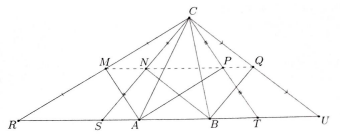
\includegraphics[scale=0.75]{img/img001.png}
    
    \item \iniTri. Seja $H$ seu ortocentro. Os pontos $L$ e $P$ são as projeções de $H$ sobre as bissetrizes interna e externa de $\angle ACB$, respectivamente. Prove que os pontos $M$, $L$ e $P$ são colineares, onde $M$ é o ponto médio de $AB$. \dica %Paralelogramos %Conjugados isogonais %Marque ângulos
    
    \item \iniTri. Uma reta passando por $C$ intersecta a bissetriz interna de $A$ e o circuncírculo de $\Delta ABC$ nos pontos $M$ e $N$, respectivamente. Uma circunferência $k_1$ passa por $A$ e toca $CM$ nos pontos $P$ e $Q$, respectivamente. Prove que os pontos $N$, $P$ e $Q$ são colineares. \dica %Marcação de ângulos
    
    \item Seja $\angle AOC$ um ângulo. O ponto $B$ fica sobre a semirreta $OA$ e o ponto $D$ fica sobre a semirreta $OC$. Além disso, $AB=CD$, $A$ fica entre $O$ e $B$, e $C$ fica sobre $O$ e $D$. Os circuncírculos de $\Delta ADO$ e $\Delta BOC$ intersectam-se novamente no ponto $K$. Prove que $OK$ é bissetriz interna de $\angle AOC$. \dica %Marque ângulos %Semelhança de triângulos %Definição de bissetriz
    
    \item Seja $ABC$ ($AC>BC$) um triângulo, seja $CL$ ($L\in AB$) sua bissetriz interna, e seja $O$ seu circuncentro. Denote os circuncentros de $\Delta ALC$ e $\Delta BLC$ por $O_1$ e $O_2$, respectivamente. Prove que $OO_1=OO_2$. \dica %Marcação de ângulos %Lei dos Senos %Lei dos Cossenos
    
    \item \iniTri. Seja $CL$ ($L\in AB$) uma bissetriz interna. O incírculo de $\Delta ALC$ toca $AC$, $AL$ e $CL$ nos pontos $M$, $N$ e $P$, respectivamente, e o $C$-exincírculo de $\Delta BCL$ toca as retas $BL$, $CB$ e $CL$ nos pontos $Q$, $R$ e $S$, respectivamente. Prove que cada uma das triplas de pontos $M$, $N$, $S$ e $P$, $Q$, $R$ são colineares. \dica %Trigonometria %Teorema do Bico %Teorema de Menelaus
    
    \item \iniTri. Sejam $AA^{\prime}$ e $BB^{\prime}$ alturas e $k$ o incírculo centrado em $I$. As retas $AI$ e $BI$ intersectam $BC$ e $AC$ nos pontos $F$ e $G$ respectivamente. A circunferência $k$ toca $BC$ e $CA$ nos pontos $D$ e $E$ respectivamente. Se $A^{\prime}B^{\prime}\cap GF=X$, prove que os pontos $E$, $D$ e $X$ são colineares. \dica %Razão anarmônica %Teorema de Tales %Teorema da bissetriz %Semelhança de triângulos
    
    \item \iniTri. Seja $CL$ bissetriz interna e $I$ incentro. A mediatriz do segmento $CL$ intersecta as bissetrizes internas de $\angle BAC$ e $\angle ABC$ nos pontos $M$ e $N$, respectivamente. Prove que o quadrilátero $MINC$ é cíclico. \dica %Marcação de ângulos
    
    \item \iniTri. Seja $I$ seu incentro. Os pontos $Y\in AI$ e $X\in BI$ são escolhidos de forma que $\angle XCA=\angle YCB$. Prove que as retas $AX$, $CI$ e $BY$ são concorrentes. \dica %Teorema de Desargues %Aplique razões em áreas %Teorema da bissetriz %Teorema de Ceva
    
    \item \iniTri. Sejam $AM$ e $BN$ bissetrizes internas que se intersectam em $I$. Pontos $L$ e $K$ são escolhidos sobre a reta $AB$ tais que $LN$ e $CN$ são simétricas com respeito a $BN$, e tais que $CM$ e $KM$ são simétricas com respeito a $AM$. Seja $D=LN\cap KM$. Prove que $DI\perp AB$. \dica %Marque ângulos %Exincentro %Deduza que $I$ é incentro de outro triângulo
    
    \item Seja $ABC$ ($AC>BC$) um triângulo de alturas $AA_1$ e $BB_1$, que se intersectam no ponto $H$. As bissetrizes internas de $\angle HAC$ e $\angle HBC$ se intersectam no ponto $L$. Sejam $M$ e $N$ os pontos médios de $AB$ e $CH$, respectivamente. Prove que os pontos $M$, $L$ e $N$ são colineares. \dica %Marque ângulos
    
    \item \iniTri. Seja $C_2$ o ponto médio de $AB$. As retas tangentes ao circuncírculo de $\Delta ABC$ em $A$ e $B$ se intersectam no ponto $N$. Prove que $\angle ACC_2=\angle BCN$. \dica %Aplique várias leis dos senos
    
    \item \iniTri. Os pontos $D$ e $E$ são escolhidos sobre os lados $AC$ e $BC$ de tal forma que o quadrilátero $ABED$ é cíclico. Seja $M$ o ponto médio de $AB$ e seja $F$ a interseção das retas tangentes ao circuncírculo de $\Delta DEC$ nos pontos $D$ e $E$. Prove que os pontos $M$, $F$ e $C$ são colineares. \dica %Conjugadas isogonais %Semelhança de triângulos %Marcação de ângulos
    
    \item \iniTri. Seja $k$ seu circuncírculo. As retas tangentes a $k$ por $A$ e $B$ se intersectam no ponto $D$. Digamos que $CD$ intersecte $k$ uma segunda vez no ponto $E$. As projeções de $E$ sobre $AB$, $BC$ e $CA$ são $N$, $P$ e $M$, respectivamente. Prove que $N$ é o ponto médio de $PM$. \dica %Reta de Simson %Lei dos senos
    
    \item \iniTri. As retas tangentes a seu circuncírculo pelos pontos $A$ e $B$ se intersectam em $T$. A reta $CT$ intersecta o circuncírculo de $\Delta ABC$ uma segunda vez no ponto $D$. Seja $CL$ ($L\in AB$) bissetriz interna de $\angle ACB$. Prove que $DL$ é bissetriz interna de $\angle ADB$. \dica %Simedianas %Ache um quadrilátero harmônico %Teorema da bissetriz interna
    
    \item \iniTri. As retas tangentes ao seu circuncírculo pelos pontos $A$ e $B$ se intersectam em $T$. A reta $CT$ intersecta o circuncírculo de $\Delta ABC$ uma segunda vez no ponto $D$. Seja $E$ a reflexão de $D$ com respeito a $AB$, e seja $M$ o ponto médio de $AB$. Prove que os pontos $C$, $E$ e $M$ são colineares. \dica %Conjugadas isogonais
    
    \item \iniTri. As retas tangentes a seu circuncírculo pelos pontos $A$ e $B$ se intersectam em $T$. A reta $CT$ intersecta o circuncírculo de $\Delta ABC$ uma segunda vez no ponto $D$. Seja $N\in CD$ um ponto tal que $\angle NBC=\angle ACN$. Prove que $\angle BCN=\angle CAN$. \dica %Simediana %Ache um quadrilátero harmônico %Conjugadas isogonais
    
    \item \iniTri. Sejam $E$, $F$ e $M$ pontos médios de $AC$, $BC$ e $EF$, respectivamente. O segmento $CD$ é uma altura de $\Delta ABC$. Prove que os circuncírculos de $\Delta ECF$, $\Delta BDF$ e $\Delta ADE$ concorrem num ponto da reta $DM$. \dica %Ponto fantasma %Marcação de ângulos %Congruência de triângulos
    
    \item \iniTri. Seja $M$ o ponto médio de $AB$ e seja $D$ o ponto de interseção das retas tangentes ao circuncírculo de $\Delta ABC$ pelos pontos $A$ e $B$. As projeções de $D$ sobre as retas $CA$ e $CB$ são $E$ e $F$, respectivamente. Prove que $CM\perp EF$. \dica %Ache um quadrilátero cíclico %Seja $H=CM\cap EF$ %Marcação de ângulos
    
    \item \iniTri. Seja $N$ o ponto médio da altura $CD$ e seja $M$ o ponto médio de $AB$. Seja $L$ o ponto de Lemoine de $\Delta ABC$. Prove que os pontos $N$, $L$ e $M$ são colineares. \dica %Propriedades do ponto de Lemoine %Teorema de Steiner
    
    \item Seja $k$ uma circunferência. Um ponto $C$ é escolhido exterior a $k$. As retas tangentes $k$ por $C$ tocam a circunferência nos pontos $A$ e $B$. Prove que o incentro de $\Delta ABC$ fica sobre $k$. \dica %Marcação de ângulos %Definição do incentro
    
    \item As circunferências $k_1$ e $k_2$ se tocam externamente no ponto $I$. Sejam $l_1$ e $l_2$ as retas tangentes externas comuns às duas circunferências. Os pontos de tangência de $l_1$ e $l_2$ a $k_2$ são $A$ e $B$, respectivamente. Os pontos de tangência de $l_1$ e $l_2$ a $k_1$ são $D$ e $C$, respectivamente. Prove que o quadrilátero $ABCD$ é inscritível. \dica %Use o problema anterior %Angle chasing
    
    \item \iniTri. $I$ é o incentro do triângulo. O incírculo de $\Delta ABC$ toca $AB$ em $N$. O $C$-exincírculo de $\Delta ABC$ toca $AB$ em $M$. Sejam $P$ e $Q$ as projeções ortogonais de $A$ e $B$ sobre a reta $CI$, respectivamente. Prove que os pontos $P$, $M$, $Q$ e $N$ ficam sobre uma circunferência de diâmetro $MN$. \dica %Ache um quadrilátero cíclico %Marque ângulos
    
    \item \iniTri. Seja $\omega$ seu incírculo, de centro $I$. Denote a projeção ortogonal de $B$ sobre $AI$ por $K$. Sejam $N$ e $M$ os pontos tangência de $AC$ e $BC$ por $\omega$, respectivamente. Prove que os pontos $M$, $N$ e $K$ são colineares. \dica %Marque ângulos para achar um quadrilátero cíclico %Prove a colinearidade por ângulos
    
    \item \iniTri. Seja $\omega$ seu incírculo, de centro $I$. Digamos que $AB$ toque $\omega$ em $N$. Sejam $K$ e $M$ os pontos médios de $CN$ e $AB$, respectivamente. Prove que $K$, $I$ e $M$ são colineares. \dica %Teorema de Newton %Note que um triângulo pode ser interpretado como um quadrilátero degenerado
    
    \item \iniTri. Seja $k$ seu incírculo, de centro $I$. Digamos que $AB$ toque $k$ no ponto $P$. Seja $CH$ ($H\in AB$) uma altura de $\Delta ABC$. Denote o ponto médio de $CH$ por $M$. Seja $k_C(I_C)$ o $C$-exincírculo de $\Delta ABC$, e digamos que ele toque $AB$ em $F$. Prove que os pontos $M$, $I$ e $F$ são colineares, e prove que os pontos $M$, $P$ e $I_C$ são colineares. \dica %Reflita $P$ com relação a $I$ %Ache uma boa homotetia %Aplique o Teorema de Steiner num trapézio da figura   
    
    \item \iniTri. Digamos que seu incírculo toque os lados $BC$, $CA$ e $AB$ nos pontos $F$, $E$ e $D$, respectivamente. Digamos também que seu $C$-exincírculo toque as retas $BC$, $CA$ e $AB$ nos pontos $Q$, $P$ e $M$, respectivamente. Seja $MN$ ($N\in PQ$) uma altura em $\Delta PMQ$, e seja $DH$ ($D\in EF$) uma altura em $\Delta EDF$. Prove que $\angle ACN=\angle BCH$. \dica %Trigonometria
    
    \item \iniTri. Sejam $\omega_X(I_X)$ seus $X$-exincírculos para $X\in\{A,B,C\}$. Digamos que $\omega_A$ toque $AB$, $AC$ e $BC$ em $P$, $Q$ e $E$, respectivamente, assim como $\omega_B$ toca $BC$, $BA$ e $CA$ em $N$, $M$ e $D$, respectivamente. Diremos ainda que $PE\cap MN=R$ e $MD\cap PQ=S$. Prove que os pontos $I_B$, $R$, $C$, $S$ e $I_A$ são colineares. \dica %Marcação de ângulo %Lei dos Senos
    
    \item \iniTri. Sejam $\omega_X(I_X)$ seus $X$-exincírculos para $X\in\{A,B,C\}$. Digamos que $\omega_A$ toque $AB$, $AC$ e $BC$ em $P$, $Q$ e $E$, respectivamente, assim como $\omega_B$ toca $BC$, $BA$ e $CA$ em $N$, $M$ e $D$, respectivamente. Seja $PE\cap MD=F$. Prove que $CF=r$, onde $r$ é o inrraio de $\Delta ABC$. \dica %Marque ângulos e aplique Lei dos Senos
    
    \item \iniTri. Sejam $\omega_X(I_X)$ seus $X$-exincírculos para $X\in\{A,B,C\}$. Digamos que $\omega_A$ toque $AB$, $AC$ e $BC$ em $P$, $Q$ e $E$, respectivamente, assim como $\omega_B$ toca $BC$, $BA$ e $CA$ em $N$, $M$ e $D$, respectivamente. Sejam $PE\cap MD=U$ e $PQ\cap MN=F$. Prove que $CF\perp AB$ e que $CU\perp AB$. \dica %Marque ângulos %Lei dos Senos %Observe $\Delta MPF$
    
    \item \iniTri. Sejam $\omega_X(I_X)$ seus $X$-exincírculos para $X\in\{A,B,C\}$. Digamos que $\omega_A$ toque $BC$ em $N$, assim como $\omega_B$ toca $CA$ em $M$ e $\omega_C$ toca $CA$ e $CB$ em $P$ e $Q$, respectivamente. Prove que as retas $PQ$, $MN$ e $AB$ concorrem. \dica %Teorema de Menelaus
    
    \item \iniTri. Seja $K$ o ponto médio de $AB$. A reta $CL$ ($L\in AB$) é a bissetriz interna de $\angle ACB$. O $B$-exincírculo de $\Delta ABC$ toca $AC$ no ponto $N$. O $A$-exincírculo de $\Delta ABC$ toca $BC$ no ponto $P$. Seja $M$ ponto médio de $NP$. Prove que $KM\parallel CL$. \dica %Marcação de ângulo %Base média %Teorema da Bissetriz
    
    
    
    
    
    
    
    
    
    
    
    
    
\end{enumerate}
\end{multicols}


\end{document}























